\subsection{Bolometric IR Luminosity Density} \label{Sec: IR Density}
In this section, we calculate and analyse the bolometric IR (8-1000$\mu$m) luminosity density (LD) and star formation rate density ($\rho_{SFRD}$). Figure \ref{Fig: SFRD} shows the IR LD ($\rho_{IR}$) of our ZFOURGE and CIGALE results with values in table \ref{Tab: SFRD}. At each redshift bin, $\rho_{IR}$ is calculated by integrating under the best fitting luminosity function with equation \ref{EQ: Luminosity Density}:

\begin{equation} 
    \rho_{IR} = \frac{1}{\ln(10)} \int_{0}^{\infty} \varphi(L) dL 
    \label{EQ: Luminosity Density}
\end{equation}

Where $\phi(L)$ is the best fitting luminosity function (The Saunders function: Equation \ref{EQ: Saunders Function}). We utilise \texttt{scipy.integrate.quad} \citep{virtanen_scipy_2020} which uses an adaptive quadrature algorithm automatically subdividing the integration interval and applying a recursive Simpson’s rule. We perform the integration from $0$ to $\infty$ $L_{\odot}$ by cumulatively summing the integrand at incremental bounds (e.g. from $10^{10}$ to $10^{12}$ $L_{\odot}$, $10^{12}$ to $10^{14}$ $L_{\odot}$, etc) because the quadrature algorithm isn't well suited for small areas over very large bounds. In practice, additional calculations of $\rho_{IR}$ above $10^{20}$ $L_{\odot}$ are negligible. To generate $\rho_{IR}$ uncertainty values, we re-perform the integration using the LF fit errors.

\begin{figure*}[t!]
    \centering
    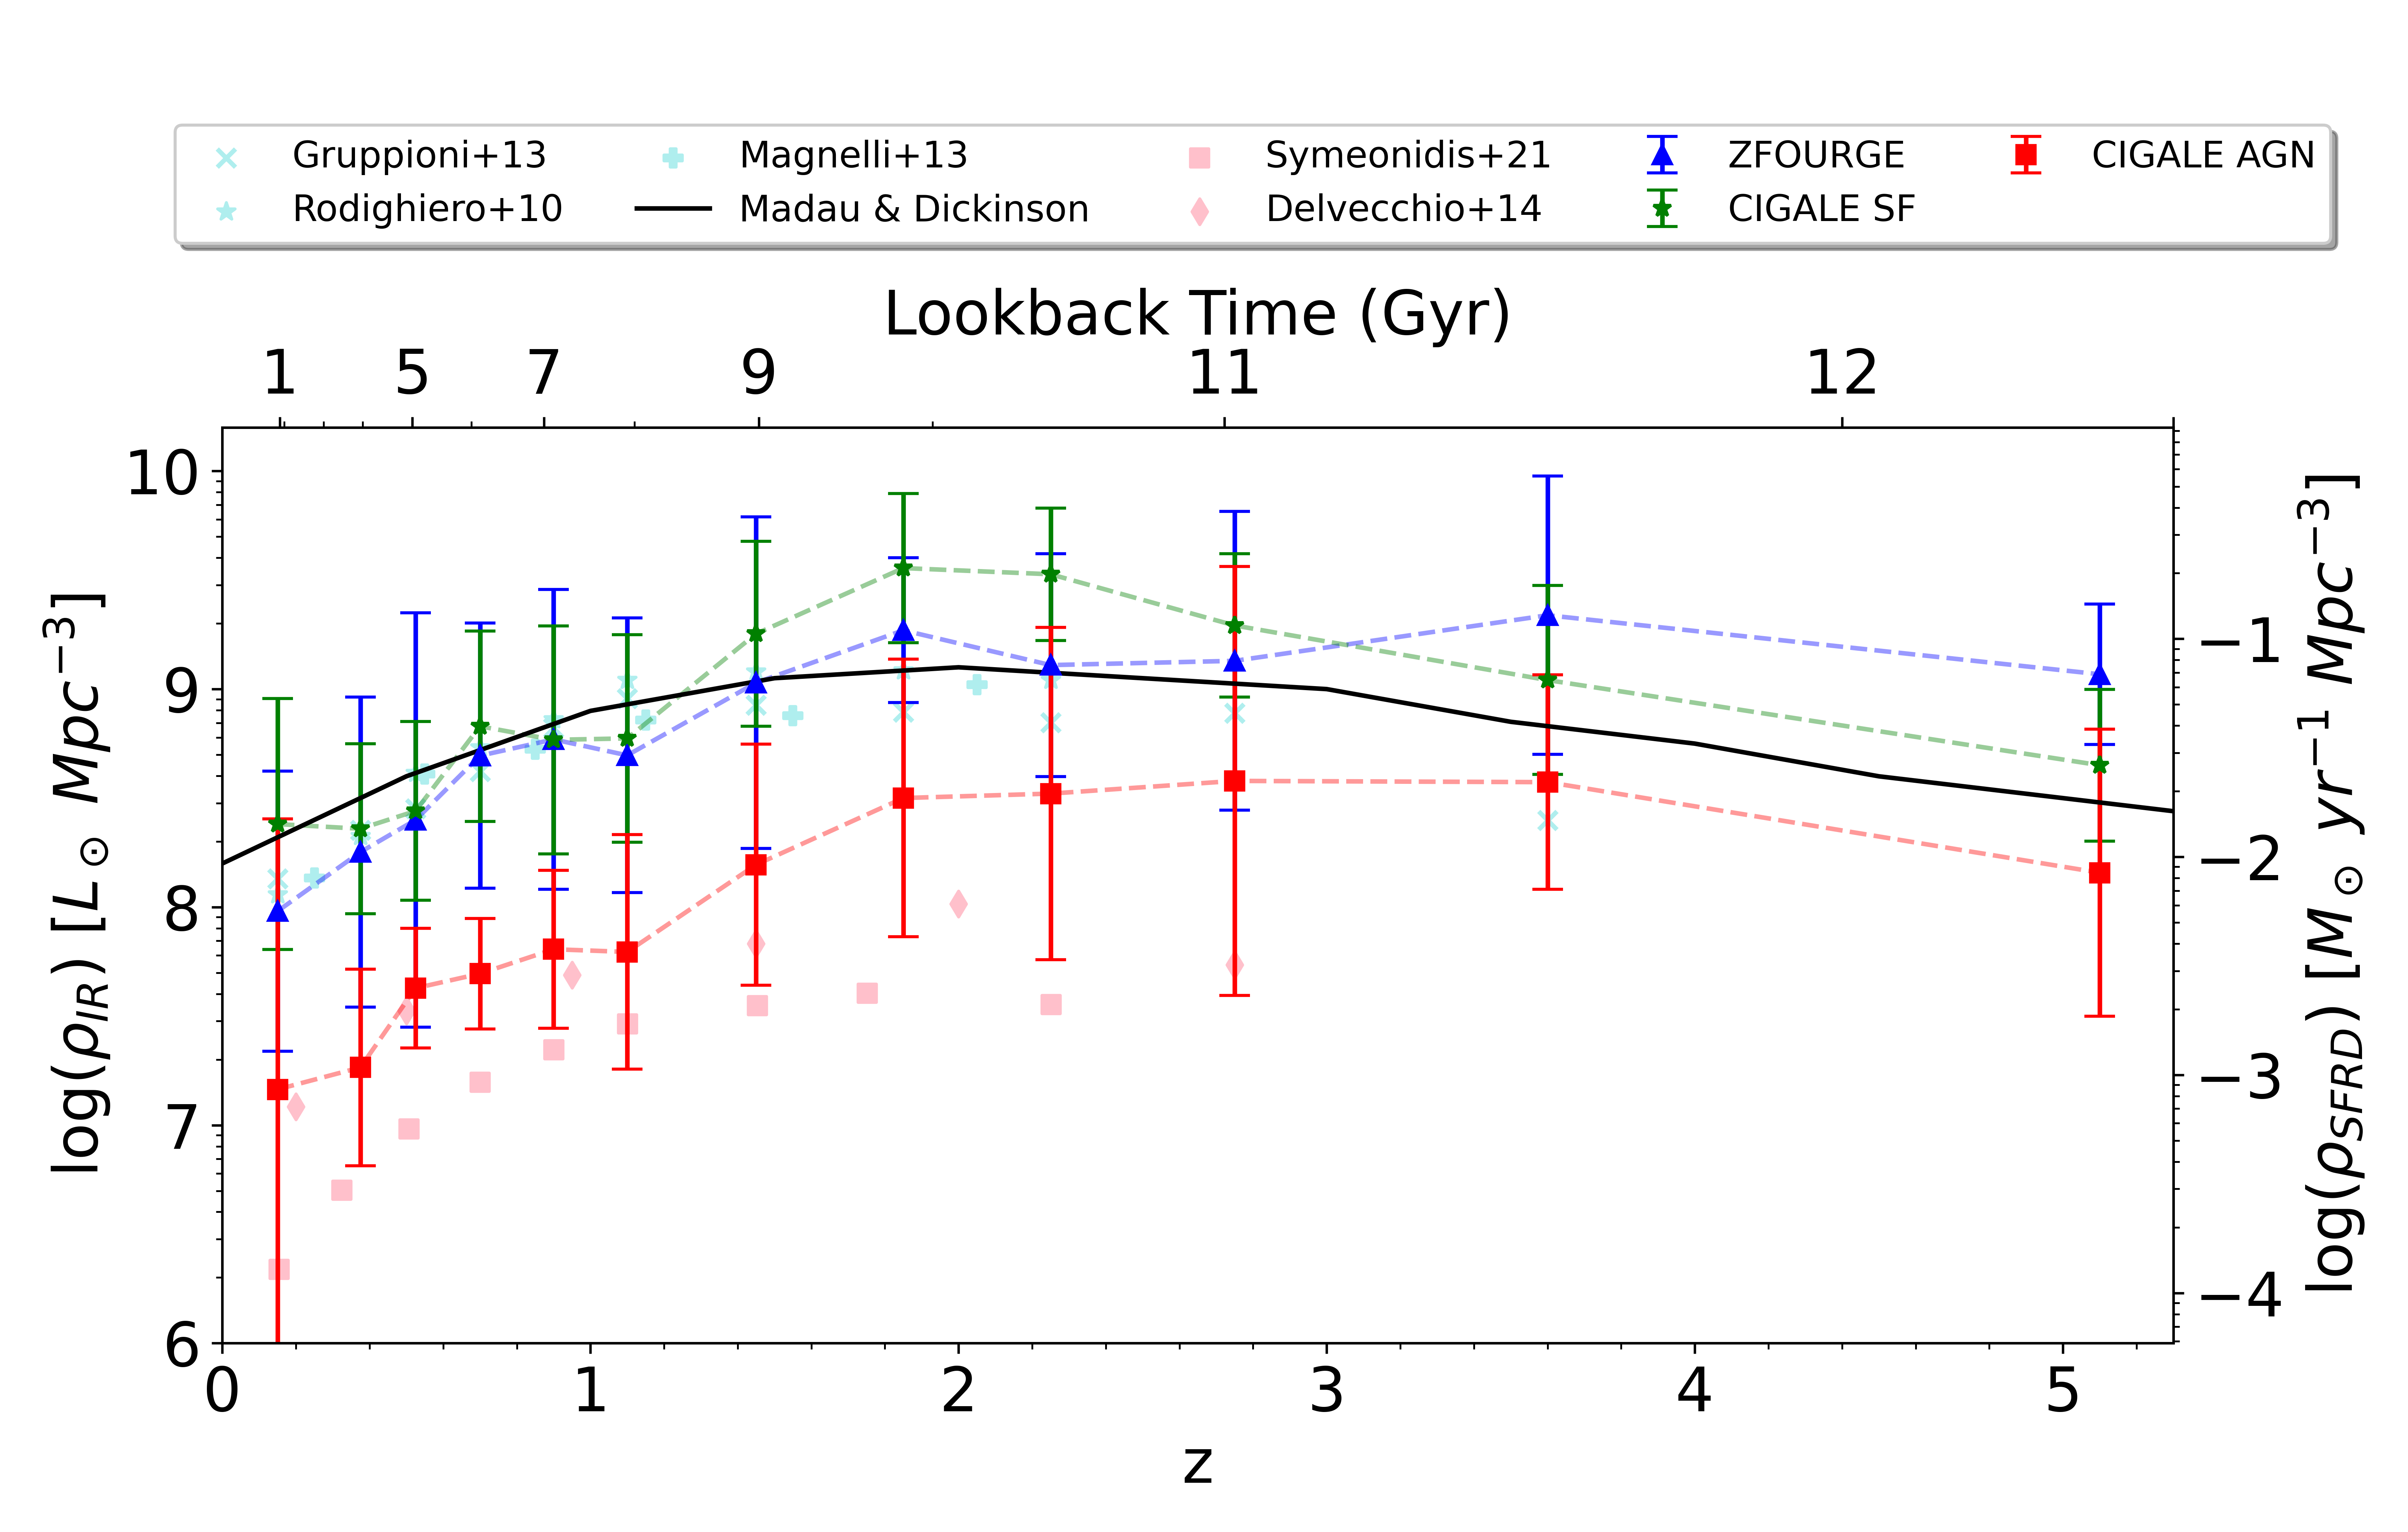
\includegraphics[width=\textwidth]{Figures/SFRD.png}
    \caption{Evolution of the IR luminosity density (LD) calculated by integrating under the best fitting LFs. Uncertainties are calculated by re-performing the integration with errors from the LF fitting process. Blue triangles represent ZFOURGE; green stars CIGALE SF; and red squares CIGALE AGN. The right side y-axis is obtained from \cite{kennicutt_global_1998} based on a Salpeter IMF with $\rho_{SFRD} = \rho_{IR} \times 1.7\times10^{-10} \ L_{\odot}$. The top axis shows the lookback time in billions of years. We compare our results with relevant literature. \cite{gruppioni_herschel_2013, rodighiero_mid-_2010, magnelli_deepest_2013} as light blue compare the SF LD. \cite{symeonidis_agn_2021} and \cite{delvecchio_tracing_2014} as light red compare the AGN LD. The solid black line is the \cite{madau_cosmic_2014} LD.}
    \label{Fig: SFRD}
\end{figure*}

\begin{figure*}
    \centering
    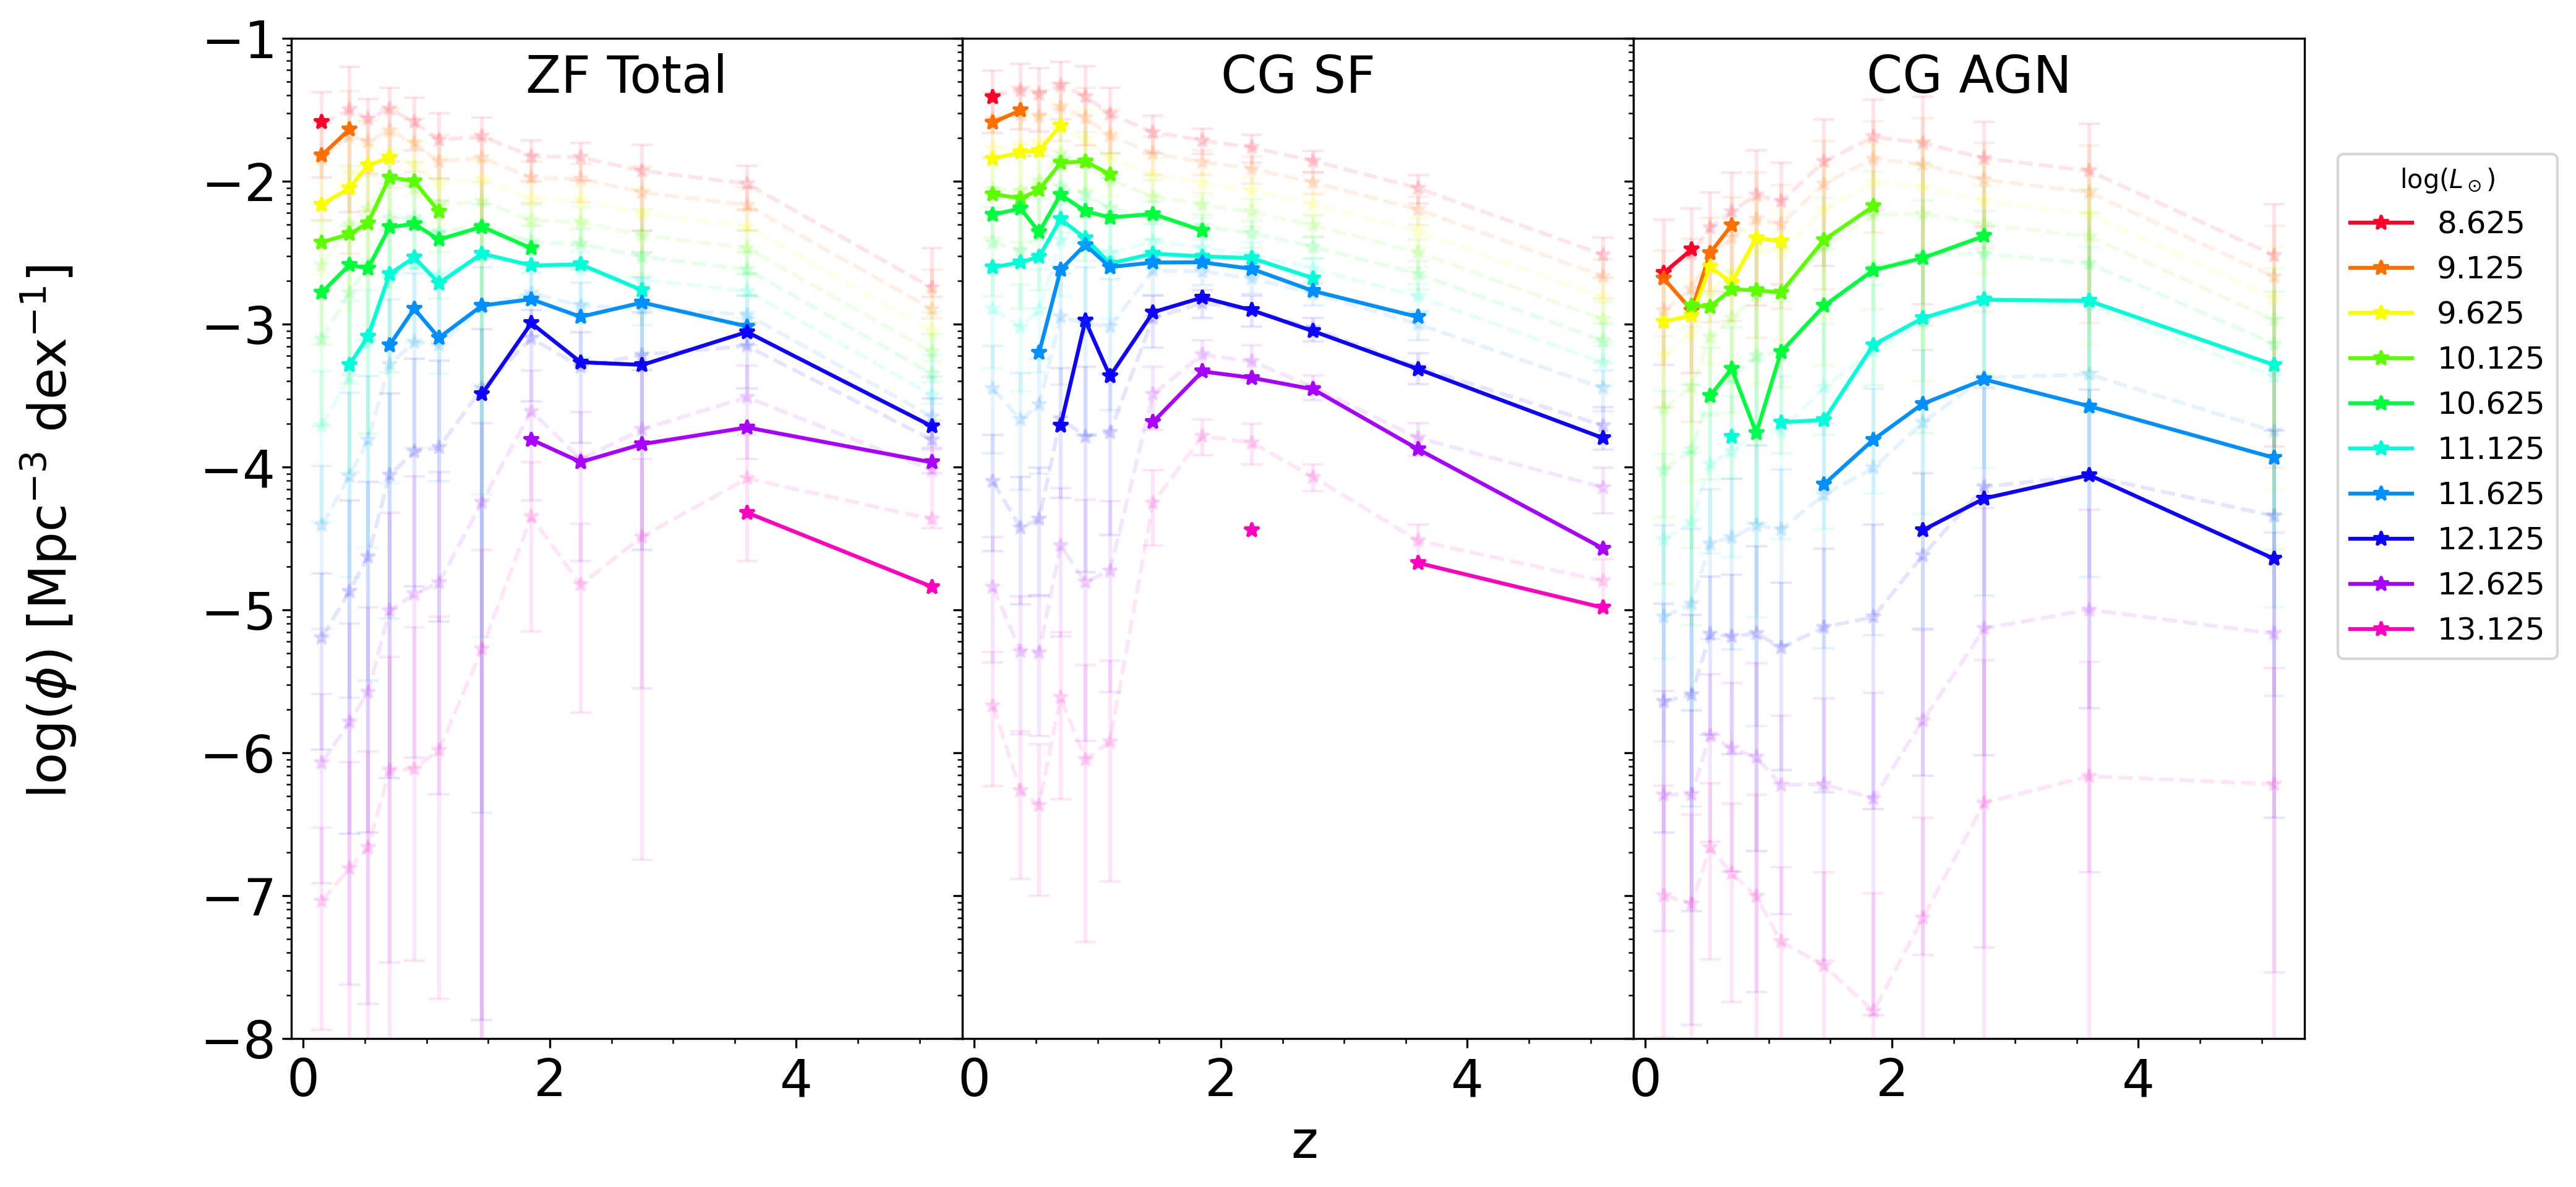
\includegraphics[width=\textwidth]{Figures/Class_Evo.png}
    \caption{Luminosity class evolution as a function of redshift. $\phi$ values connected by straight lines correspond to real values in Figure \ref{Fig: Bolometric IR LF}. $\phi$ values connected by dashed lines are estimated from the best fitting LF. Error bars represent the propagated uncertainty derived from the LF. Real luminosity classes are 0.25 log$(L_{\odot})$ in width and centred in the middle (e.g. 8.5 --- 8.75 is centred on 8.625). Estimated classes are calculated at the centre of the luminosity bin (e.g. 8.625). Not all luminosity bins from Figure \ref{Fig: Bolometric IR LF} are displayed to reduce clutter.}
    \label{Fig: Class Evo}
\end{figure*}

The secondary right-hand-side axis of figure \ref{Fig: SFRD} displays the conversion to SFRD provided by \cite{kennicutt_global_1998} based on a Salpeter IMF calculated with $\rho_{SFRD} = \rho_{IR} \times 1.7\times10^{-10} L_{\odot}$. We remind the reader that the IR AGN densities do not have an associated SFR. The top x-axis shows the lookback time in billions of years, placing the evolution of the universe in the context of time to showcase the important evolutionary epochs.

Our ZFOURGE results in figure \ref{Fig: SFRD} show rapid evolution from $0<z<2$. From $z>2$ onwards, there is essentially no evolution as $\rho_{IR}$ remains roughly constant. As discussed in section \ref{Sec: Parameter Evolution}, our highest redshift bin was thought to suffer from incompleteness, but our $\rho_{IR}$ values are still high. We see excellent agreement with the literature from $0<z<2$ but deviate significantly from $z>2$ onwards. Importantly, we do not find a turnover in the IR LD at $z\approx2$ for ZFOURGE. This is a different result than is often published in the literature (\citealp{gruppioni_herschel_2013, magnelli_deepest_2013, madau_cosmic_2014, lutz_far-infrared_2014} and references within). However, this is not a new result as is seen in \cite{rodighiero_mid-_2010}, but they do not probe to a sufficiently high enough redshift to capture the decline above $z>2$.

The CIGALE decomposed SF IR LD is seen to increase from $0<z<2$ and decline from $z>2$ onwards. This agrees well with the literature, especially \cite{madau_cosmic_2014}. However, at $z>2$, our CIGALE results are elevated by $\approx 1.3$x. Some of this elevation can be attributed due to the higher bright-end slope $(\sigma = 0.7)$ compared to the literature $(\sigma = 0.5)$ (e.g. \citealp{gruppioni_herschel_2013}). However, this is not the sole reason. Likely due to poor FIR constraints, the luminosity is overestimated. As mentioned in Section \ref{Sec: ZF Total Discussion}, a drop in literature LFs is noticeable at $1.7\leq z< 2.0$. However, we do not find this drop in either the ZFOURGE or CIGALE datasets. Subsequently, $\rho_{IR}$ is elevated at $1.7\leq z< 2.0$ even when the bright end slope is reduced.  

The ability of CIGALE to recover the turnover in the SF $\rho_{IR}$, where ZFOURGE does not, suggests that CIGALE is effectively isolating the SF component and lends confidence to the accuracy of our results. The CIGALE SF LD is slightly elevated over ZFOURGE at most redshift bins. We believe this is not an error on CIGALE's part, but likely the FIR-poor ZFOURGE data it is based on. We find excellent agreement with the literature up until $z=2$. As mentioned previously in section \ref{Sec: Bolometric IR LF}, both \cite{fu_decomposing_2010} and \cite{wu_mid-infrared_2011} argue that when AGN are removed, the luminosity function is better fit with a Schechter function. Our CIGALE SF LF instead applies the Saunders function so that the CIGALE AGN and ZFOURGE LFs can be directly compared. This may also explain why our CIGALE SF LFs (figure \ref{Fig: Bolometric IR LF}) are elevated, as integrating under the Schechter functions results in a slight drop in $\rho_{IR}$. Furthermore, the uncertainties are almost all within the range of \cite{madau_cosmic_2014}.

The CIGALE AGN LD (or $\Psi_{BHAR}$) follows a similar evolution to the literature, though it is elevated, likely due to CIGALE's ability to detect fainter AGN. The trend seen in the CIGALE SF LD increasing from $0<z<2$ and declining from $z>2$ is still present, but not clear. This is not the first time a turnover in the AGN $\rho_{IR}$ has been seen. \cite{symeonidis_agn_2021} presents their IR AGN densities up to $z\approx2.5$. These results are at most $\approx 1$ order of magnitude lower than ours. We attribute this to their use of \cite{aird_evolution_2015} X-ray sources, which are converted to optical luminosity and then to IR luminosity. Their X-ray-selected galaxies likely miss the highly obscured and faint-luminosity counterpart that this work recovers. As \cite{symeonidis_agn_2021} only extends as far as $z\approx2.5$, the AGN $\rho_{IR}$ turnover is poorly defined. AGN by \cite{delvecchio_tracing_2014} agrees well with our results. We recalculated the AGN $\rho_{IR}$ for the \cite{delvecchio_tracing_2014} dataset because they did not provide $\rho_{IR}$ values in their work, instead focusing on the black hole accretion rate density ($\Psi_{bhar}$). Using the function parameters they reported, we use the same integration method described previously to calculate $\rho_{IR}$ and find good agreement with our results. Again, we attribute elevated densities to CIGALE's ability to recover fainter AGN.

Both \cite{symeonidis_agn_2021} and \cite{delvecchio_tracing_2014} show AGN LD peaks at $z\approx2$, but are poorly defined. Our CIGALE AGN LD peaks sometime between $z\approx2.5-3.5$. As was mentioned in section \ref{Sec: Parameter Evolution}, there appeared to be a significant evolutionary epoch for AGN occurring below sometime $z\approx2$ and this is reflected in our AGN LD results. From $0<z<2$, AGN density is seen to decline. Relying solely on the LD evolution of AGN and SF galaxies to assess their overall evolution may oversimplify their complex evolution. The functional fits have likely smoothed out slight variations in the LF, potentially masking essential details. 

% In the first $\approx$ 6 Gyrs of the universe ($z>1$), CIGALE AGN and SF LD evolution are positively correlated. In this case, AGN and SF LD evolve together and at the same time. 

% It is also possible that AGN activity peaks $\approx1$ Gyr before SF. This would point towards at a delayed AGN feedback scenario. In this case, declining AGN activity positively influences SFR with a time delay in between \textcolor{red}{(cite).}.

% In conjunction with our CIGALE SF LD, this implies a scenario in which AGN activity and SF evolve concurrently.

% Similar parameter evolution was seen in \cite{delvecchio_tracing_2014}, although they only have three redshift bins at or below $z=1$. 

% As mentioned, the turnover in the IR LD is hotly debated \citep{magnelli_deepest_2013}. However, 